According to Theorem~\ref{structure thm}, we have the generating function for the quasi-consecutive pattern $\sigma k$, where $k$ is the largest element, provided the generating function for $\sigma$ is known. In this section, we derive an explicit generating function for one of the patterns, namely $\underline{123}$, and subsequently for $\underline{321}$ as well, thanks to Proposition~\ref{omega--omega^c}. The approach we use is the so-called generalized run theorem; see Theorem~\ref{thm:gen run thm}. For the remaining four patterns, $\underline{132}$, $\underline{213}$, $\underline{231}$, and $\underline{312}$, we demonstrate that their generating functions satisfy certain partial differential equations, as presented in Subsection~\ref{subsec:g.f.132}.

\subsection{The run theorem} \label{subsec:run theorem}


In this subsection we use Zhuang's generalized \emph{run theorem} \cite{zhu16} to get two generating functions. Here ``run'' refers to a maximal weakly increasing consecutive subsequence in a word, so naturally this theorem suits the increasing pattern $\underline{123}$ the best. But according to Proposition~\ref{omega--omega^c}, finding the Eulerian distribution over $\underline{123}$-avoiding permutations is equivalent to finding the Eulerian distribution over $\underline{321}$-avoiding permutations. And the bivariate generating function for $\underline{321}$-avoiding permutations is already known to be \cite{MR06}

\begin{align}\label{Sn321des}
	\sum_{n\geq 0}\dfrac{x^n}{n!}\sum_{\pi \in S_n(\underline{321})} t^{\mathrm{des}(\pi)}=\dfrac{\mathrm{e}^{x/2}\sqrt{1-4t}}{\sqrt{1-4t}\cosh {\left(\frac{x}{2}\sqrt{1-4t}\right)}-\sinh{\left(\frac{x}{2}\sqrt{1-4t}\right)}}.
\end{align}
See also \cite[Thm.~5.3.4]{kit11}. Our proof of the following result could thus be viewed as an alternative approach to deriving \eqref{Sn321des}. We only sketch a proof here using the run theorem and illustrate the associated ``run network'' in Fig.~\ref{sn123runnetwork}. To make the paper self-contained however, we provide some preliminary definitions and facts in the Appendix, and the reader is referred to Zhuang's original paper~\cite{zhu16} for further information.

Note that a permuation $\pi$ avoids the consecutive pattern $\underline{123}$ if and only if each run of $\pi$ has length 1 or 2. Therefore, the corresponding run network is given by Fig.~\ref{sn123runnetwork}.

% , and we assign the weights $w_1^{(1 , 1)}=w_2^{(1,1)}=t$.

\begin{figure}[htbp]	
	 \centering
		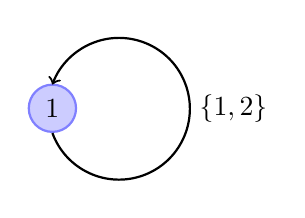
\begin{tikzpicture}
			[phase/.style ={circle,draw=blue!50,fill=blue!20,thick,inner sep=0pt, minimum size=6mm}]
			\node (A) at (0,-2) [phase] {1};
			\node (C) at (2.3,-2) {$\{1,2\}$};
			\draw[->,thick] (A.south) arc[start angle=-160, end angle=160, radius=9mm];
		\end{tikzpicture}
\caption{Run network for permutations avoiding consecutive pattern $\underline{123}$.}
\label{sn123runnetwork}
\end{figure}

\begin{theorem}
\begin{align}\label{Sn(123)des+1}
1+\sum_{n\geq 1}\dfrac{x^n}{n!}\sum_{\pi \in \S_n(\underline{123})} t^{\mathrm{des}(\pi)+1}=\dfrac{\mathrm{e}^{tx/2}\sqrt{t-4}}{\sqrt{t-4}\cosh {\left(\frac{x}{2}\sqrt{t^2-4t}\right)}-\sqrt{t}\sinh{\left(\frac{x}{2}\sqrt{t^2-4t}\right)}},
\end{align}
equivalently, we have
\begin{align}\label{Sn(123)des}
	\sum_{n\geq 0}\dfrac{x^n}{n!}\sum_{\pi \in \S_n(\underline{123})} t^{\mathrm{des}(\pi)}=\dfrac{t^{-1}\mathrm{e}^{tx/2}\sqrt{t-4}}{\sqrt{t-4}\cosh {\left(\frac{x}{2}\sqrt{t^2-4t}\right)}-\sqrt{t}\sinh{\left(\frac{x}{2}\sqrt{t^2-4t}\right)}}-\dfrac{1}{t}+1.
\end{align}
\end{theorem}

\begin{proof}
According to Fig.~\ref{sn123runnetwork} and applying Theorem~\ref{thm:gen run thm}, the inverse of $1+xt+x^2t$ is enumerator of those permutations whose increasing runs are no more than 2, and each increasing run is weighted by $t$. Next we proceed to seek the exponential generating function expression of $$\frac{1}{1+xt+x^2t}$$ with respect to the variable $x$. Since 
$$\dfrac{1}{1+xt+xt^2}=\dfrac{t-4+\sqrt{t^2-4t}}{2\left(t-4\right)}\dfrac{1}{1-\frac{2tx}{-t+\sqrt{t^2-4t}}}+\dfrac{t-4-\sqrt{t^2-4t}}{2(t-4)}\dfrac{1}{1-\frac{2tx}{-t-\sqrt{t^2-4t}}},$$ 
the exponential generating function turns out to be 
$$\frac{t-4+\sqrt{t^2-4t}}{2\left(t-4\right)} \mathrm{Exp}\left(\frac{-tx-x\sqrt{t^2-4t}}{2}\right)+\frac{t-4-\sqrt{t^2-4t}}{2\left(t-4\right)} \mathrm{Exp}\left(\frac{-tx+x\sqrt{t^2-4t}}{2}\right)$$
whose inverse simplifies to the desired expression \eqref{Sn(123)des+1}.
\end{proof}

% We note in passing that Eq.~\eqref{Sn(123)des} could be viewed as a bivariate extension of the expression of $P(0,z)$ in \cite[Thm.~4.1]{EN03}, which is the generating function of permutations avoiding $\underline{123}$.

%Note that $\pi^r \in \S_n(\underline{321})$ and $\mathrm{des}(\pi^r)=n-1-\mathrm{des}(\pi)$ if $\pi \in \S_n(123)$, consequently we have following result.
% By Proposition~\ref{omega--omega^c}, we immediately have the following result.
% \begin{corollary}	
% \begin{align}\label{Sn321des}
% 	\sum_{n\geq 0}\dfrac{x^n}{n!}\sum_{\pi \in S_n(\underline{321})} t^{\mathrm{des}(\pi)}=\dfrac{\mathrm{e}^{x/2}\sqrt{1-4t}}{\sqrt{1-4t}\cosh {\left(\frac{x}{2}\sqrt{1-4t}\right)}-\sinh{\left(\frac{x}{2}\sqrt{1-4t}\right)}}.
% \end{align}
% \end{corollary}


\subsection{The generating functions involving partial differential equations} \label{subsec:g.f.132}
Noting the equivalences implied by Proposition~\ref{omega--omega^rc}: $\underline{312} \overset{\des}{\sim }\underline{231} $, $\underline{213} \overset{\des}{\sim }\underline{132}$, and the relation $\underline{231}=(\underline{132})^r$, it suffices to compute the generating function for one of the patterns, say $\underline{132}$.

Let $U_n(t)$ (resp., $V_n(t)$) denote the generating function of the permutations $\pi$ of length $n$ that avoid the pattern $\underline{132}$ and start with an ascent $\pi_1 < \pi_2$ (resp., a descent $\pi_1 > \pi_2$), where $t$ tracks the descent number of $\pi$.
We define $U = U(x,t) := \sum_{n \geq 0} U_n(t) \frac{x^n}{n!}$ and $V = V(x,t) := \sum_{n \geq 0} V_n(t) \frac{x^n}{n!}$, with the initial terms given by $U_0(t) = U_1(t) = V_0(t) = V_1(t) = 0$.

\begin{proposition} \label{132}
The bivariate generating functions $U$ and $V$ satisfy the partial differential equations:
    \begin{align*}
    \dfrac{\partial U}{\partial x} &=(tU+1)(U+x+1)-1,\\
    \dfrac{\partial V}{\partial x} &=t(V+x)(U+x+1).
    \end{align*}
    Moreover,
    \begin{align*}
    A^{\underline{132}}(x,t)=A^{\underline{213}}(x,t)=1+x+U(x,t)+V(x,t).
    \end{align*}
\end{proposition}

\begin{proof}
    Let $\pi \in \S_{n+1}(\underline{132})$. Considering the position of $1$ as illustrated in Fig.~\ref{fig:position of 1}, we obtain
    \begin{equation}\label{eqn-prop-4-6}U_{n+1}(t)=tU_n(t)+tnU_{n-1}(t)+t\sum_{i=2}^{n-2}\binom{n}{i}U_i(t)U_{n-i}(t)+U_{n}(t),\quad n \ge 3.\end{equation}

    \begin{figure}[ht]
        \centering
        \begin{tikzpicture}
            \draw (0,0)--(5,0);
            \foreach \I in {0,0.5,...,5}
            {\draw (\I,0)--(\I,0.15);}
            \node at (4.75,0.3) {$1$};
        \end{tikzpicture}

        \begin{tikzpicture}
            \draw (0,0)--(5,0);
            \foreach \I in {0,0.5,...,5}
            {\draw (\I,0)--(\I,0.15);}
            \node at (4.25,0.3) {$1$};
        \end{tikzpicture}

        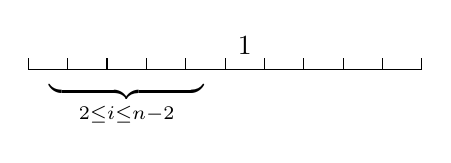
\begin{tikzpicture}
            \draw (0,0)--(5,0);
            \foreach \I in {0,0.5,...,5}
            {\draw (\I,0)--(\I,0.15);}
            \node at (2.75,0.3) {$1$};
            \node at (1.25,-0.3) {$\underbrace{\phantom{a+b+c+d}}_{2 \le i\le n-2}$ };
        \end{tikzpicture}

        \begin{tikzpicture}
            \draw (0,0)--(5,0);
            \foreach \I in {0,0.5,...,5}
            {\draw (\I,0)--(\I,0.15);}
            \node at (0.25,0.3) {$1$};
        \end{tikzpicture}
        \caption{Position of $1$ in $\pi \in \S_{n+1}(\underline{132})$}\label{fig:position of 1}
    \end{figure}
Multiplying by $\dfrac{x^n}{n!}$ both sides of (\ref{eqn-prop-4-6}) and summing over all $n\geq 3$, we have    

\begin{align*}
    \sum_{n\ge 3}U_{n+1}(t)\frac{x^n}{n!}={}&t\sum_{n\ge 3}U_n(t)\frac{x^n}{n!}+tx\sum_{n\ge 3}U_{n-1}(t)\frac{x^{n-1}}{(n-1)!} \\
    &+t\sum_{n\ge 3}\sum_{i=2}^{n-2}\binom{n}{i}U_i(t)U_{n-i}(t)\frac{x^n}{n!}+\sum_{n\ge 3}U_n(t)\frac{x^n}{n!} \\
    ={}& t\sum_{n\ge 3}U_n(t)\frac{x^n}{n!}+tx\sum_{n\ge 2}U_{n}(t)\frac{x^{n}}{n!} \\
    &+t\sum_{n\ge 3}\sum_{i=0}^{n}\binom{n}{i}U_i(t)U_{n-i}(t)\frac{x^n}{n!}+\sum_{n\ge 3}U_n(t)\frac{x^n}{n!} \\
    ={}& t\left(U-\frac{x^2}{2}\right)+txU+tU^2+\left(U-\frac{x^2}{2}\right).
\end{align*}

Note that $U_2(t)=1$ and $U_3(t)=1+t$. Hence,  
\begin{align*}
    \sum_{n\ge 3}U_{n+1}(t)\frac{x^n}{n!}&=\frac{\partial }{\partial x}\left(U-\frac{x^2}{2}-(1+t)\frac{x^3}{3!}\right) = \frac{\partial U}{\partial x}-x-(1+t)\frac{x^2}{2} \\
    &=t\left(U-\frac{x^2}{2}\right)+txU+tU^2+\left(U-\frac{x^2}{2}\right).
\end{align*}

Therefore, $\dfrac{\partial U}{\partial x}=x+tU+txU+tU^2+U=(tU+1)(U+x+1)-1$.
Using Mathematica, we obtain the expansion $U(x,t)=\dfrac{x^2}{2}+(1+t)\dfrac{x^3}{3!}+(1+5t+t^2)\dfrac{x^4}{4!}+(1+16t+10t^2+t^3)\dfrac{x^5}{5!}+(1+42t+71t^2+16t^3+t^4)\dfrac{x^6}{6!}+(1+99t+399t^2+197t^3+23t^4+t^5)\dfrac{x^7}{7!}+\cdots$.


Similarly, we have
$$V_{n+1}(t)=tV_n(t)+tnV_{n-1}(t)+t\sum_{i=2}^{n-2}\binom{n}{i}V_i(t)U_{n-i}(t)+tnU_{n-1}(t),\quad n\ge 3.$$
Note that $V_2(t)=t$ and $V_3(t)=2t+t^2$. Repeating the above computations for $V$, we have


\begin{align*}
    \sum_{n\ge 3}V_{n+1}(t)\frac{x^n}{n!}={}& t\sum_{n\ge 3}V_n(t)\frac{x^n}{n!}+tx\sum_{n\ge 3}V_{n-1}(t)\frac{x^{n-1}}{(n-1)!} \\
    &+t\sum_{n\ge 3}\sum_{i=2}^{n-2}\binom{n}{i}V_i(t)U_{n-i}(t)\frac{x^n}{n!}+tx\sum_{n\ge 3}U_{n-1}(t)\frac{x^{n-1}}{(n-1)!} \\
    ={}& t\sum_{n\ge 3}V_n(t)\frac{x^n}{n!}+tx\sum_{n\ge 2}V_{n}(t)\frac{x^{n}}{n!} \\
    &+t\sum_{n\ge 3}\sum_{i=0}^{n}\binom{n}{i}V_i(t)U_{n-i}(t)\frac{x^n}{n!}+tx\sum_{n\ge 2}U_{n}(t)\frac{x^{n}}{n!} \\
    ={} & t\left(V-\frac{tx^2}{2}\right)+txV+tUV+txU.
\end{align*}
Then,
\begin{align*}
    \sum_{n\ge 3}V_{n+1}(t)\frac{x^n}{n!} &= \frac{\partial }{\partial x}\left(V-t\frac{x^2}{2}-(2t+t^2)\frac{x^3}{3!}\right)=\frac{\partial V}{\partial x} -tx-tx^2\left(1+\frac{t}{2}\right) \\
    &=t\left(V-\frac{tx^2}{2}\right)+txV+tUV+txU.
\end{align*}

Therefore, $\dfrac{\partial V}{\partial x}=tx+tx^2+tV+txV+tVU+txU=t(V+x)(U+x+1)$.
Using Mathematica, $V(x,t)=t\dfrac{ x^2}{2}+(2t+t^2)\dfrac{x^3}{3!}+(3t+5t^2+t^3)\dfrac{x^4}{4!}+(4t+21t^2+9t^3+t^4)\dfrac{x^5}{5!}+\cdots$.
\end{proof}

\begin{corollary}\label{231}
We have
    \begin{align*}
    A^{\underline{231}}(x,t)=A^{\underline{312}}(x,t)=\dfrac{1}{t} \left(U(xt,\dfrac{1}{t})+V(xt,\dfrac{1}{t})\right)+x+1.
    \end{align*}
\end{corollary}

\begin{proof}
    Applying Proposition~\ref{omega--omega^c}, we obtain
    \begin{equation*}
    A^{\underline{231}}(x,t)=\dfrac{1}{t} \left(A^{\underline{132}}(xt,\dfrac{1}{t})-1\right)+1=\dfrac{1}{t} \left(xt+U(xt,\dfrac{1}{t})+V(xt,\dfrac{1}{t})\right)+1. \qedhere
    \end{equation*}
\end{proof}

